%%%%%%%%%%%%%%%%%%%%%%%%%%%%%%%%%%%%%%%%%%%%%%%%%%%%%%%%%%%%%%%%%%%%%%%%%%%%%%%%%
%
% Purpose:  Mathematical Formulation part of Product Spec for the RadiationPressure model
%
%
%%%%%%%%%%%%%%%%%%%%%%%%%%%%%%%%%%%%%%%%%%%%%%%%%%%%%%%%%%%%%%%%%%%%%%%%%%%%%%%%

\section{Mathematical Formulations}\label{sec:mathformulations}

 \subsection{Reduction of Flux by Intervening Body}\label{ref:shadowcalculator}
 The flux algorithm is qualitatively described in the section
 \textref{calculate\_flux}{ref:calculateflux}.
 The mathematical treatment of flux starts with a trivial inverse-square-law
 application to obtain a raw flux.  A secondary calculation then identifies
 whether that flux is being eclipsed by an intervening body.  This section
 covers that identification, and some of the easier cases.  The intricate
 calculations to determine the fractional eclipse that occurs in a scenario
 in which a part of the solar disk is eclipsed are described in the next
 section (the \textref{Conical Eclipse Calculator}{sec:conicaleclipsecalculator}).

 The \textref{Process Architecture}{sec:processarchitecture}
 contains flow charts (see, in particular, Figures~\ref{fig:flow_calculate_shadow}
 and~\ref{fig:flow_third_body_adjustments}) that assist
 in interpreting the interdependence of these methods.

\subsubsection{Introduction to Problem}
  Suppose that we have a spacecraft orbiting a planet, and that the
  reference frame in which the position of the spacecraft is known is
  arbitrarily oriented, but planet{}-centered.

  Suppose further that the planet is being illuminated by a flux with
  vector \  $\vec{\phi }=\phi \hat{\phi }=\phi \; [\phi _{1},\phi _{2},\phi
  _{3}]$ in that same reference frame, and that the spacecraft is at a
  position  $[x,y,z]$.
  \bigskip
  \bigskip
  \begin{figure}[!ht]
  \begin{center}
    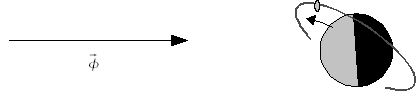
\includegraphics[height=20mm]{figs/shadow/shadow_seeker_fig1.jpg}
    \end{center}
    \caption{Shadowing overview}
    \label{fig:shadow_seeker1}
  \end{figure}

  Define a new coordinate system, \textit{ $\hat{a},\hat{b},\hat{c}$
  }, such that  $\hat{a}$ is oriented with the
  solar flux vector $\vec{\phi}$ for the planet (i.e. from the sun to the
  planet), and $\hat{b}$ and $\hat{c}$ form a
  plane perpendicular to the sun.

  The origin of this coordinate system is concentric with the
  inertial system, so that
  $|\vec{r}_{\mathit{xyz}}|=|\vec{r}_{\mathit{abc}}|$ .
  The new system should be right{}-handed, so that
  $\hat{b}\times \hat{c}=\hat{a}$ .

  The orientation of the \textit{b}{}- and
  \textit{c}{}- axes is arbitrary, and there are an infinity of
  possibilities for such a coordinate system.  However, because we have
  axial symmetry, it is not necessary to define these axes.
  The position vector can, instead, be expressed in terms of two components --
  one parallel, and one perpendicular, to the flux vector.

  \bigskip

  $\vec{r}$ represents the position of the vehicle with respect to the
  shadow body.

  $\vec{d}$ represents the position of the vehicle with respect to the
  sun.

  $r,d$ represent the magnitudes of  $\vec{r},\vec{d}$ respectively.

  \bigskip

  Then the components of the position vector that are parallel and perpendicular
  to the flux vector are (respectively):

  $r_\Vert\ =\ \vec{r}\cdot \hat{\phi }$

  $r_\bot\ =\ \sqrt{r^{2}-r_\Vert^{2}}$

  NOTES
  \begin{itemize}
   \item $r_\Vert \leqslant  0$ places the vehicle on the sunward side of
   the planet.
    In this case, there can be no eclipse.
   \item $r_\Vert > 0$ places the vehicle on the shadow-side of the planet.
    In this case, the determination of whether there is an eclipse depends
    on the value of $r_\bot$.
  \item $r_\bot > 0$ always; the positive square root is taken.
  \end{itemize}


  \bigskip

  \subsubsection{Cylindrical shadowing}\bigskip

  The simplest consideration is one in which the planet casts a
  cylindrical shadow.

  \begin{figure}[!ht]
    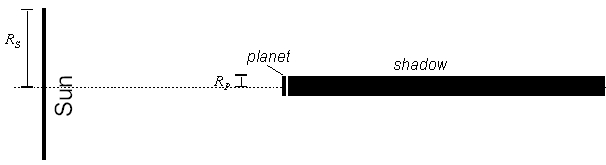
\includegraphics[height=40mm]{figs/shadow/shadow_seeker_fig2.jpg}
    \caption{Cylindrical shadow geometry}
    \label{fig:shadow_seeker2}
  \end{figure}

  \bigskip
  If the spacecraft is in a position such that
  $r_\Vert>0$ and
  $r_\bot<R_{P}$ , then it will be in 100\% shadow.
  \ Otherwise, it will be 100\% illuminated.

  \bigskip

  \clearpage
  \subsubsection{Conical shadowing}\bigskip
  A more complicated scenario is to consider the more realistic conical
  shadow:

  \begin{figure}[!ht]
    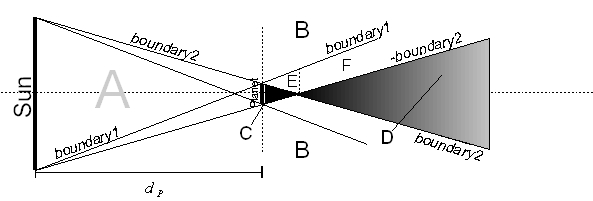
\includegraphics[height=50mm]{figs/shadow/shadow_seeker_fig3.jpg}
    \caption{Conical shadow geometry}
    \label{fig:shadow_seeker3}
  \end{figure}

   \bigskip


   The following sequence of diagrams may help with visualization of the how
   the relative positions of a planet and the sun might change as a vehicle
   moves across the eclipse field.  For this sequence, consider Figure
   \ref{fig:shadow_seeker3} with a vehicle moving from bottom to to through
   regions B-F-D-F-B.
   \begin{itemize}


    \item {}-boundary 1 (B-F): the circle of the planet and
   that of the sun make first contact
   
\includegraphics{figs/shadow/shadow_seeker_fig4.jpg}

    \item boundary 2 (F-D): the planet disk is completely contained
   within the solar disk~~~
   
\includegraphics{figs/shadow/shadow_seeker_fig5.jpg}

    \item {}-boundary2 (D-F): the planet disk begins to leave the
   solar disk~~~~~~~~~~~~~~~~~~~~~~~~
   
\includegraphics{figs/shadow/shadow_seeker_fig6.jpg}

    \item boundary1 (F-B): the two circles separate~~~~~~~~~~~~~~~~~~~~~~~~~~~~~~~~~~
   ~~~~~~~~~~~~~~~~~~
   
\includegraphics{figs/shadow/shadow_seeker_fig7.jpg}

   \end{itemize}
   \bigskip

   The same sequence could also describe a similar path, from top to bottom,
   moving through regions B-E-C-E-B

   \begin{itemize}

   \item boundary 1 (B-E): the circle of the planet and that of the sun make
   first contact

   \item boundary 2 (E-C): the planet disk completely covers the solar disk

   \item {}-boundary2 (C-E): the solar disk starts to emerge from behind the
   planet disk

   \item {}-boundary1 (E-B): the two circles separate

   \end{itemize}


   The two boundaries can be represented as simple lines, $y=mx+b$.
   The gradient for the two boundaries is easily evaluated using the
   distance between the sun and planet, $d_P$.
   \begin{itemize}
    \item boundary1: $\frac{R_P+R_S} {d_P}$
    \item boundary2: $\frac{R_P-R_S} {d_P}$
   \end{itemize}
   The y-intercept for both boundaries is $R_P$.

   Thus, the two boundaries are defined by the relations:
   \begin{itemize}
    \item boundary1: $r_\bot=\left(\frac{R_{P}+R_{S}}{d_{P}}\right)r_\Vert+R_{P}$
    \item boundary2: $r_\bot=\left(\frac{R_{P}-R_{S}}{d_{P}}\right)r_\Vert+R_{P}$
   \end{itemize}


   For the purposes of algebra, let  $b_{1}$  and
    $b_{2}$ represent the values of
   $r_\bot$ that would lie on boundary 1 and boundary
   2, respectively, at some value of  $r_\Vert$ .

   \textbf{Region A} of Figure \ref{fig:shadow_seeker3}, is characterized by
   $r_\Vert<0$.  In this region there will never be any shadow and the full
   disk is counted.


   \textbf{Region B} of Figure \ref{fig:shadow_seeker3} is characterized by
    $r_\Vert>0$ and $r_\bot \geqslant b_{1}$.  In this region, the full disk
    will be counted.

    NOTES:
    \begin{itemize}
     \item $r_\bot>b_{1} \implies r_\bot d_P \geqslant (R_P + R_S)
            r_\Vert + R_P d_P $
    \end{itemize}



   \textbf{Region C} of Figure \ref{fig:shadow_seeker3} is characterized by
   $r_\Vert>0$ and $r_\bot \leqslant b_{2}$.  In this region, the eclipse is
   total; none of the disk will be counted,  $I=0$.

   NOTES:
   \begin{itemize}
    \item $r_\bot<b_{2} \implies r_\bot d_P \leqslant (R_P - R_S) r_\Vert
          + R_P d_P$
    \item Because $R_P < R_S$ (typically) and $r_\bot \geqslant 0$, this becomes
          impossible at large $r_\Vert$, as expected.
   \end{itemize}



   \textbf{Region D} of Figure \ref{fig:shadow_seeker3} is characterized by
   $r_\Vert>0$ and $r_\bot \leqslant -b_{2}$.  In this region, the eclipse will
   be annular, and a function of $r_\Vert$ only (i.e. independent of $r_\bot$).

   NOTES:
   \begin{itemize}
    \item $r_\bot \leqslant -b_{2} \implies r_\bot d_P \leqslant (R_S - R_P)
           r_\Vert - R_P d_P$
    \item For modeling shadowing from a source other than the sun, it could
          be possible to have $R_P > R_S$.  In this case, the left hand side
          of the inequality is positive and the right-hand-side negative-definite.
          The inequality cannot be satisfied and region D is not available.
   \end{itemize}


   In the diagram below, the white circle represents the solar disk, and the
   shaded circle the intervening planetary disk.

   
\includegraphics{figs/shadow/shadow_seeker_fig8.jpg}

   The planetary angular size is  $\frac{2R_{P}}{r}$
   and the solar angular size is  $\frac{2R_{S}}{d}$ .

   The area of the disk is proportional to the square of the angular size;

   hence the planetary disk obscures
   $\left(\frac{R_{P} \cdot d}{R_{S} \cdot r}\right)^{2}$ of the solar disk,

   and the illumination becomes
   \begin{equation*}
   I=1-\left(\frac{R_{P} \cdot d}{R_{S} \cdot r}\right)^{2}
   \end{equation*}

   \bigskip

   \textbf{Region E} of Figure \ref{fig:shadow_seeker3} is characterized by
   $(r_\Vert>0)$ and $(r_\bot>b_{2})$ and $r_\bot<b_{1}$ and
   $\frac{R_P}{r} > \frac{R_S}{d}$.  In this
   region, the eclipse will be partial, transitioning to total.  The magnitude of
   the eclipse effect will be a function of both $r_\Vert$ and $r_\bot$.  The
   resulting illumination will transition from 100\% on
   boundary1 to 0\% on boundary2.

   NOTES:
   \begin{itemize}
    \item Algorithmically, this set of constraints is acheived when the tests
          for regions A-D have failed and $R_P \cdot d > R_S \cdot r$
   \end{itemize}

   In the diagram below, the white circle
   represents the solar disk, and the shaded circle the intervening planetary disk.

   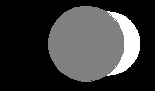
\includegraphics{figs/shadow/shadow_seeker_fig9.jpg}

   The mathematical treatment of this transition is described in
   subsection \ref{sec:conicaleclipsecalculator}.

   \bigskip

   \textbf{Region F} of Figure \ref{fig:shadow_seeker3} is characterized by
   $(r_\Vert>0)$ and $(r_\bot>b_{2})$ and $r_\bot<b_{1}$ and
   $\frac{R_P}{r} \geqslant \frac{R_S}{d}$.
   In this
   region, the eclipse will be partial, transitioning to annular.  The magnitude of
   the eclipse effect will be a function of both $r_\Vert$ and $r_\bot$.  The
   resulting illumination will transition from 100\% on
   boundary1 to the value determined for region D on (-)boundary2.

   NOTES:
   \begin{itemize}
    \item Algorithmically, this set of constraints completes the set.  It is
          achieved when tests for all other regions have failed.
   \end{itemize}


   
\includegraphics{figs/shadow/shadow_seeker_fig10.jpg}
   The mathematical treatment of this transition is described in
   subsection \ref{sec:conicaleclipsecalculator}.

   \bigskip

   \subsubsection{The flux unit{}-vector}\bigskip

   The direction of the flux acting on the spacecraft in full illumination
   is going to be on a line from the center of the sun reference frame to
   the center of pressure of the spacecraft (or, in the case of a
   representation in terms of multiple facets, the desired vectors
   would be to the center of pressure of each facet).
   The center of pressure of each facet is
   defined relative to the structural reference frame in the Surface Model.

   When the sun is partially obscured, the origin of the flux vector will
   be shifted slightly from the center of the sun to the center of
   radiation, as shown in the diagram below, with the cross representing the
   center of radiation of the partially obscured solar disk.

   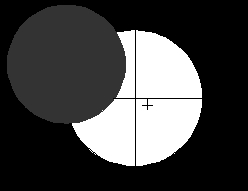
\includegraphics{figs/shadow/shadow_seeker_fig11.jpg}

   If we were to be concerned with the consequential change in direction of the
   flux vector, it would no longer be sufficient to work in the
   axially symmetric, two{}-dimensional system just developed.
   Instead, a full 3{}-dimensional treatment would be required, which would
   add significant computational expense, with minimal impact on the results.
   The radiation pressure is a relatively small force, and the
   effect of the deviation of the direction of the flux vector over such
   small angles is negligible compared to other approximations being made.

   The direction of the flux vector is therefore assumed to be on the
   direction from the center of the sun to some reference point on the
   spacecraft.  Which reference point should be used is not particularly
   relevant for the purposes of determining this direction; using the
   wrong reference point will have even less of an effect than using the
   wrong center of radiation for the source.  Consequently, the same flux
   vector will be used for all of the facets that make up the vehicle.

  \subsection{Conical Eclipse Calculator}\label{sec:conicaleclipsecalculator}

   This subsection describes the method used for calculating the extent of
   shadowing for partial spacecraft shadowing cases, such as would occur in
   in regions E and F of Figure \ref{fig:shadow_seeker3}.

   \bigskip
   \subsubsection{Definitions}


   The front body (the eclipsing body) will be given the subscript
   \textit{1.}

   The rear body (the sun) will be given the subscript \textit{2.}

   The term ``radius'', as used in this description, is not always intended
   to represent the physical radius, but often
   the angular radius, as observed from the point of interest. Reference
   will be made to places where the radius of the planet is larger than
   that of the sun. This does not imply that the planet must be
   physically larger, just that it occupies a larger solid angle due to
   its relative proximity.
   Typically, linear distances are represented by Roman lettering (R, r) and
   angles by Greek lettering ($\theta, \psi, \phi$).
   Ultimately though, we are looking for a fractional area, so both the linear
   and angular sizes will become moot.

   \subsubsection{Introduction}

   Figure \ref{fig:shadow_calc1} shows the area of the shaded subsection of a
   circle, defined by angle  $\theta $ and radius \textit{R}.  It can be
   expressed as
   \begin{equation*}
    A = R^2 (\theta - sin \theta cos \theta)
   \end{equation*}


   \begin{figure}[!ht]
   \begin{center}
    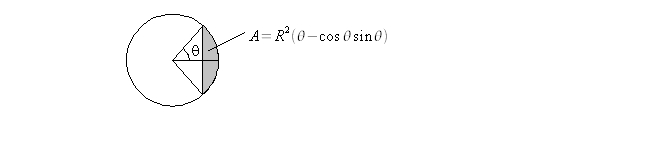
\includegraphics[height=45mm]{figs/shadow/shadow_calculator_fig1.jpg}
    \end{center}
    \caption{The area of the segment of a circle}
    \label{fig:shadow_calc1}
   \end{figure}

   For two intersecting circles, the area can be identified by considering it as
   a sum of two such two circle segments,
   as shown in Figure~\ref{fig:shadow_calc2}~:

   \begin{figure}[!ht]
   \begin{center}
    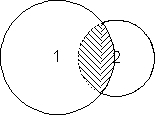
\includegraphics[height=40mm]{figs/shadow/shadow_calculator_fig2.jpg}
    \end{center}
    \caption{The area of overlap of two circles, decomposed into two segments}
    \label{fig:shadow_calc2}
   \end{figure}

   In this diagram, the shaded area on the left
   (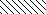
\includegraphics{figs/shadow/shadow_calculator_fig3.jpg})
   is attributed to the circle on the right (labeled 2), while the area on the
   right
   (
\includegraphics{figs/shadow/shadow_calculator_fig4.jpg}), is attributed to
   the circle on the left (labeled 1).
   The total shaded area is then:

   \begin{equation*}
   A\ =\ A_{1}+A_{2}\ =\ {R_{1}}^{2}(\theta _{1}-\cos \theta _{1}\sin
   \theta _{1})+{R_{2}}^{2}(\theta _{2}-\cos \theta _{2}\sin \theta _{2})
   \end{equation*}

   \subsubsection{Direct Computation Method}

   The desired output value is the fraction of this area with respect to the
   area of the solar disk.  Without loss of generality, assign subscript $2$
   to the solar disk and subscript $1$ to the planetary disk.  Use upper-case
   $R_i$ to represent the size of the disk, lower-case $r_i$ to represent the
   distance to the disk, and $\psi_i$ to represent the angular radius of the
   disk.
   \begin{equation*}
     \psi_i = \frac{R_i}{r_i}
   \end{equation*}

   Assign variables to the ratio of angular radii and area:

   \begin{align*}
   \rho &= \frac{\psi_1}{\psi_2} \\
   \alpha &= \frac{A}{\pi R_2^2}
   \end{align*}

   Thus the fractional area $\alpha$ can be expressed in terms of $\rho$ and
   $\theta_i$, independent of $R_i$, $r_i$, and $\psi_i$:
   \begin{equation*}
    \alpha = \frac{1}{\pi} \left( \rho^2(\theta_1 - sin \theta_1 cos\theta_1) +
             \theta_{2}-\cos \theta _{2}\sin \theta _{2} \right)
   \end{equation*}

   To compute the angles $\theta_i$, we start with a triangle with vertices at
   the two disk centers and one of the points of intersection, as shown in Figure
   \ref{fig:shadow_calc_triangle}.

   \begin{figure}[!ht]
   \begin{center}
    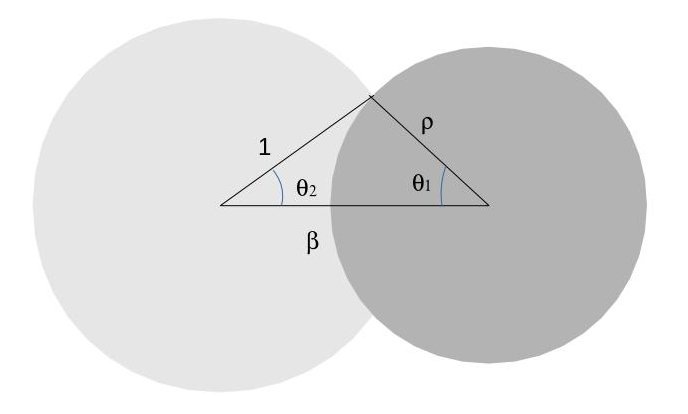
\includegraphics[height=40mm]{figs/shadow/shadow_calculator_fig6.jpg}
    \end{center}
    \caption{The scaled angular sizes of the two disks.}
    \label{fig:shadow_calc_triangle}
   \end{figure}





   The scaled separation between the disk centers is
   \begin{equation*}
     \beta = cos \theta_2 + \rho cos \theta_1
   \end{equation*}
   The perpendicular distance from the line joining the
   centers to the intersection of the two circles is
   \begin{equation*}
     sin \theta_2 = \rho sin \theta_1
   \end{equation*}

   Consequently, the values of $\theta_i$ can be determined:
   \begin{align*}
     \rho^2 cos^2 \theta_1 &= (\beta - cos \theta_2)^2 \\
     \rho^2 cos^2 \theta_1 &= \rho^2 (1 - sin^2 \theta_1) =
                               \rho^2 - sin^2 \theta_2 =
                               \rho^2 -1 + cos^2 \theta_2 \\
     (\beta - cos \theta_2)^2 &= \rho^2 -1 + cos^2 \theta_2  \\
     cos \theta_2 &= \frac{\beta^2 + 1 - \rho^2}{2s} \\
     cos \theta_1 &= \frac{\beta^2 - 1 + \rho^2}{2s \rho}
   \end{align*}

   This still requires an expression for the scaled separation ``distance'',
   $\beta$.  The angle $\phi$  between the two centers can be obtained
   from the cosine rule:

   \begin{equation*}
      d_P^2 = r_1^2 + r_2^2 - 2 r_1 r_2 cos \phi
   \end{equation*}

   where $r_i$ are the linear distances from the vehicle to the respective
   disk-centers, and $d_P$ is the linear distance between disk centers.
   $\beta$ and $\phi$ are related by the angular radius of the solar disk,
   $\psi_2$.

   \begin{equation*}
      \beta = \frac{\phi}{\psi_2} =
      \frac{cos^{-1} \left( \frac{r_1^2 + r_2^2 - d^2}{2 r_1 r_2} \right)}
           {\psi_2}
   \end{equation*}





   Notes:
   \begin{itemize}
   \item This is a cumbersome calculation, requiring
   inverse-trigonometric functions to obtain $\beta$, $\theta_1$ and
   $\theta_2$ and
   2 square-root functions to determine $sin \theta_1$ and $sin \theta_2$.
   \item The calculation $\theta_i = cos^{-1} (cos \theta_i)$ requires that $-1
   \leqslant cos \theta_i \leqslant 1$ but the expressions for
   $cos \theta_i$ have no intrinsic limit protection on them.  However,
   this requirement is handled
   within the overall model algorithm because this computation is only
   reached where $abs(1-\rho) \leqslant \beta \leqslant 1+\rho$; this constraint
   is equivalent to the necessary constraint on the value of $cos \theta_i$.
   \end{itemize}

   An alternative approach provides a very close approximation using a cubic
   polynomial of the separation distance with coefficients that are themselves
   quadratic or cubic polynomials of the ratio of the disk radii.  This
   alternative approach improves speed by a factor of approximately 4.

   \subsubsection{Alternative Representation}

     Using a system of ratios, it is straightforward to identify the extent
     of the eclipse between none and maximum, where maximum occurs when the
     smaller disk is completely covered by the larger disk.
     Note - in the case where
     $R_{2}<R_{1}$, maximum eclipse is total eclipse, whereas when
     $R_{1}<R_{2}$, maximum eclipse will be when the solar disk
     completely encompasses the planetary disk.

   We can introduce $\delta$, $\delta \in [0,1]$  to represent
   the ratio of the
   current extent of the eclipse to its maximum value.

   ${\delta}$ has value \textit{0} when the limbs make first
   contact, and value \textit{1} at second contact (total occlusion).
   It is associated with the linear coverage distance
   $s =  1 + \rho - \beta$ (see  Figure
   \ref{fig:shadow_calc5}) rather than with the occluded area,
   and increases linearly with $s$.\

   Note that the distance between first contact
   and second contact is the diameter of the smaller disk.  Thus
   $s \in [0, min (2R_1,2R_{2})]$.

   \begin{figure}[!ht]
   \begin{center}
    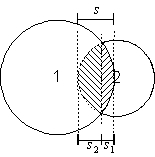
\includegraphics[height=40mm]{figs/shadow/shadow_calculator_fig5.jpg}
    \end{center}
    \caption{Overlap of two circles}
    \label{fig:shadow_calc5}
   \end{figure}

   Thus,
   \begin{equation*}
   s=
   \begin{cases}
     \delta \cdot 2R_{2}     & R_{2}<R_{1} \\
     \delta \cdot 2R_{1}     & R_{1}<R_{2}
   \end{cases}
   \end{equation*}

   In the previous section, we developed an expression for the overlap area
   as a fraction of the area of the solar disk.  Suppose, instead, we had
   developed an expression for the overlap area as a fraction of the smaller
   disk.  Let us label this new fractional area $\alpha_{-}$ and label the
   smaller radius as $R_{-}$.

   Then
   \begin{equation*}
     s = 2 \delta \cdot R_{-}
   \end{equation*}

   Note that the upper bound for $\alpha_{-}$ is independent of the
   relative sizes of the two disks (unlike the upper bound for $\alpha$).
   We always have $0 \leqslant \alpha_{-} \leqslant 1$.

   Now, with the issue associated with relative sizes set aside, we can
   obtain an expression for $\alpha_{-}$ in terms of $\delta$.

   Notice that the final desired result is still $\alpha$, and that must
   depend on whether the solar disk is smaller or larger than the
   planetary disk because we are, after
   all, looking for the fractional covering of the \textit{solar} disk.  This
   dependency can be brought back in after determining a value for
   $\alpha_{-}$:


    \begin{equation*}
     \alpha=
      \begin{cases}
       \alpha_{-} & \rho \geqslant 1 \\
       \rho ^{2}\alpha_{-} & \rho <1
      \end{cases}
    \end{equation*}


   \subsubsection{Polynomial Approximation}

    The quantity $\alpha_{-}$, for all its complexity, is a surprisingly
    well behaved function of \textit{${\delta}$} and can be
    approximated to very high
    precision with a cubic polynomial in \textit{${\delta}$}
    \begin{equation*}
     \alpha _{-}= a_{3}\delta ^{3}+ a_{2}\delta ^{2}+
    a_{1}\delta + a_{0}
    \end{equation*}

    \textbf{Value of $\delta$}

    Recall that $\delta$ is a linear function of the overlap distance, which
    is measured by $r_\bot$.  It starts with value $0$ on boundary $b_1$  at
    first
    contact and climbs to value $1$  at second contact on boundary $b_2$ (or
    $-b_2$, depending on the value of $r_\Vert$).  See Figure
    \ref{fig:shadow_seeker3} for an illustration of these two boundaries.

    Let $b_i$ represent the value of $r_\bot$ on boundary \textit{i}.  Then:

    \begin{equation*}
     \delta =
       \frac{b_1 - r_\bot}{b_1 - \left| b_2 \right|}
    \end{equation*}

    Note that the value of $b_2$ goes negative for $r_\Vert$ greater than
    some critical value, as the planetary disk becomes
    smaller than the solar disk.  To a reasonable approximation, the switch
    in sign occurs when $\rho = 1$ (this is true where $r_\bot = 0$, but
    not quite true off that axis.)

    \begin{equation*}
     \left| b_2 \right| \approx
      \begin{cases}
       b_2 & \rho \geqslant 1 \\
       -b_2 & \rho \leqslant 1
      \end{cases}
    \end{equation*}

    Thus,

    \begin{equation*}
     \delta \approx
      \begin{cases}
       \frac{b_1 - r_\bot}{b_1 - b_2} & \rho \geqslant 1 \\
       \frac{b_1 - r_\bot}{b_1 + b_2} & \rho \leqslant 1
      \end{cases}
    \end{equation*}

   The values $b_i$ can be obtained from geometry (see Figure
   \ref{fig:shadow_seeker3} for an illustration of these two boundaries)
   using simple linear expression $y = mx+b$.

   \begin{align*}
    b_1 &= m_1 r_\Vert + R_P \\
    b_2 &= m_2 r_\Vert + R_P \\
    m_1 &= \frac{R_P + R_S}{d_P} \\
    m_2 &= \frac{R_P - R_S}{d_P}
   \end{align*}

   Thus,
   \begin{equation}
     \delta \approx
      \begin{cases}
       \frac{(R_P - r_\bot) d_P + (R_P + R_S) r_\Vert}{2R_S r_\Vert} & \rho \geqslant 1 \\
       \frac{(R_P - r_\bot) d_P + (R_P + R_S) r_\Vert}{2 R_P( d_P + r_\Vert)} & \rho < 1
      \end{cases}
    \end{equation}


    \textbf{Value of the coefficients $a_i$}

    The coefficients  $a_{i}$ are themselves functions of the radius ratio
    $\rho'$ and can be approximated by quadratic or cubic functions of $\rho'$:

    \begin{equation*}
     \rho' = \frac{R_{-}}{R_{+}}=
      \begin{cases}
       \frac{1}{\rho} & \rho \geqslant 1 \\
       \rho & \rho \leqslant 1
      \end{cases}
    \end{equation*}

    Curve fitting to the analytic solution produces

    $a_{3}(\rho')=0.758656\rho^{'2}-0.0637441\rho' -1.08955$

    $a_{2}(\rho')=-1.2205\rho^{'2} -0.61815\rho' +1.629209$

    $a_{1}(\rho')=0.43723\rho^{'2}-0.529210\rho' +0.473649$

    $a_{0}(\rho')=-0.01242\rho^{'3}-0.0036715\rho^{'2}+0.0150263\rho'
    -0.0078259$

    The approximation is now complete.

    \begin{equation}
    \alpha \approx
    \begin{cases}
        \rho ^{2}\left(
        a_{3}(\rho )\cdot \delta ^{3}+
        a_{2}(\rho )\cdot \delta ^{2}+
        a_{1}(\rho )\cdot \delta +
        a_{0}(\rho )\right)     & \rho <1 \\
        a_{3}\left(\frac{1}{\rho }\right)\cdot \delta ^{3}+
        a_{2}\left(\frac{1}{\rho }\right)\cdot \delta ^{2}+
        a_{1}\left(\frac{1}{\rho }\right)\cdot \delta +
        a_{0}\left(\frac{1}{\rho }\right) & \rho \geqslant 1
    \end{cases}
    \end{equation}

    Figure \ref{fig:shadow_calc7} shows the analytic function and the
    polynomial approximation for values of

    $\rho =30,\ 2,\ 1,\ 0.75,\ 0.5,\ 0.25,\ 0.1$ .

    The analytic solution is shown as a solid line, and
    the approximation as a dotted line for each case.
    The difference between the two lines is small for all cases.


    \begin{figure}[!ht]
      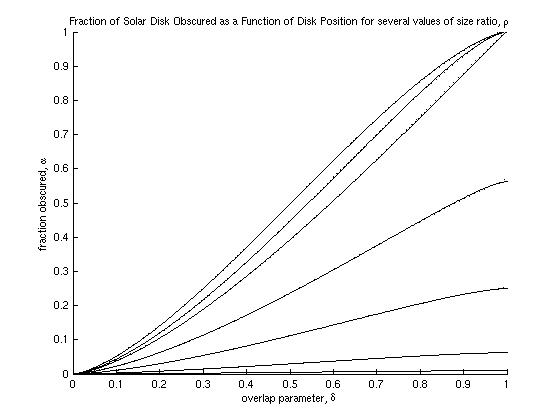
\includegraphics[height=100mm]{figs/shadow/shadow_calculator_fig7.jpg}

      \caption{Comparison of polynomial approximation to analytical solution for
      partial eclipse calculation}
      \label{fig:shadow_calc7}
    \end{figure}

   \subsubsection {Boundary Conditions and Numerical Limitations} \bigskip

    This polynomial approximation should meet certain boundary conditions;
    namely that
    \begin{equation*}
    \delta =0\Rightarrow \alpha =0
    \end{equation*}

    \begin{equation*}
      \delta = 1 \Rightarrow
      \begin{cases}
        \alpha =\rho ^{2}  &  \rho <1 \\
        \alpha =1            &  \rho \geqslant 1
      \end{cases}
    \end{equation*}

    The coefficients given are a result of best{}-fit curve{}-fitting to data
    that intrinsically included the boundary conditions, but the polynomial
    approximation does not explicitly satisfy those conditions.

    For  $\delta =0$ ,  $\alpha \in \left[-8.9\times
    10^{-3},-2.7\times 10^{-3}\right]$ . \ For small values of \textit{
    $\delta $ }, the approximated value of  $\alpha $ is less than the true
    value,
    with a maximum error of 0.89\% when  $\rho =1.0$ .

    For  $\delta =1$ and $\rho <1$,
    $\alpha =\rho ^{2}\left(-0.01242\rho
    ^{3}-0.0283\rho ^{2}+0.04022\rho +1.0054821\right)\ \in
    \ \left[1.005,1.017\right]\times \rho ^{2}$ .

    For  $\delta =1$ and $\rho >1$,
    $\alpha \in \left[1.005,1.017\right]$ ,
    For large values of\textit{ $\delta $ }, the approximated value of
    $\alpha $ is greater than the true value, with a maximum error of 1.7\% when
    $\rho =0.53$ or  $\rho =1.9$.

  \subsection{Response to Flux}\label{sec:mathform_pflux_resp}
    The interaction of matter and radiation is, to say the least, difficult to
    model.  Advances in computer graphics have produced excellent techniques
    for very finely detailed, empirically based, rendering of that interaction,
    but these techniques are typically computationally expensive, and do not
    lend themselves to efficient simulation of orbital dynamics.

    Subsection \ref{sec:mathform_pflux_resp_desc} describes the technique
    used in this model, and subsection
    \ref{sec:mathform_pflux_resp_valid} describes the validation of
    that technique.


    \subsubsection{Treatment of Flux in Calculation of Radiation
    Force}\label{sec:mathform_pflux_resp_desc}


     \begin{wrapfigure}{r}{40mm}
     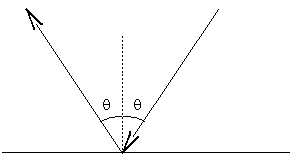
\includegraphics[width = 40mm]{figs/sda/1_sda.jpg}
     \end{wrapfigure}
     \textbf{Specular Reflection:} is the type of reflection observed
     from smooth surfaces, such as mirrors. Incident radiation is
     reflected at the same wavelength and at the same angle so that a
     clear image could, in principle, be obtained.

     \par
     \bigskip
     \bigskip
     \begin{wrapfigure}{r}{40mm}
     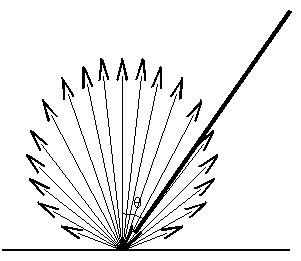
\includegraphics[width = 40mm]{figs/sda/2_sda.jpg}
     \end{wrapfigure}
     %\parpic[r]{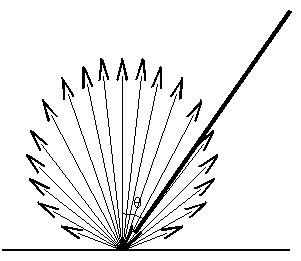
\includegraphics[width = 60mm]{figs/sda/2_sda.jpg}}
     %       \item
     \textbf{Diffuse Reflection} is the type of reflection observed
     from rough surfaces. With a reflection that is totally diffuse,
     all information about the direction of the incident radiation is
     lost, but the radiation is still reflected at the same wavelength
     as the incident radiation.
     \bigskip
     \bigskip
     \bigskip
     \bigskip
     \par
     \textbf{Absorption/Emission}: \textit{absorption} is a process by
     which the incident radiation interacts with the surface structure and
     transfers its energy and momentum to the object. This energy and
     momentum may be partially or entirely \textit{emitted,}
     spontaneously, at some later time, but may be in any direction, and
     at any wavelength. ``Some later time'' may be instantaneous.

     \begin{wrapfigure}{r}{40mm}
     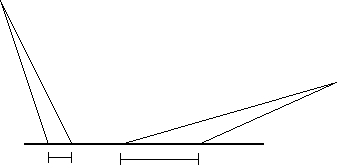
\includegraphics[width = 40mm]{figs/sda/3_sda.jpg}
     \end{wrapfigure}
     \textbf{Lambertian reflection} is a special type of
     diffuse reflection, in which the apparent brightness of the reflected
     light is constant for all viewing angles.  It is clear from the
     accompanying diagram that, when comparing the view
     through a given solid angle, an observer looking at the surface from
     an angle close to
     parallel to the plane (right side of diagram) will see more of the surface
     than an observer
     looking at the surface from an angle close to perpendicular to the plane
     (left side of diagram). If the
     emission were isotropic, the surface would appear brighter the closer
     the observer's line of sight came to being parallel
     with the plane. \ Instead, an emission profile that varies as
     $\cos \theta$ factors in the increased surface area factor
     and produces a uniform brightness for all viewing angles. One of the
     consequences of Lambertian reflection is that of axial symmetry, i.e.
     the reflected light is symmetric about the normal to the plane. For
     the purposes of momentum transfer, the integration over the full range
     of reflected light yields that Lambertian reflection is equivalent to
     absorbing the incident light and emitting 2/3 of it along the normal to
     the plane. Note that this is not true for purposes of calculating
     energy transfer. \par

     The Lambertian profile can also be used to represent the thermal
     emission from the surface; then, for an object in thermal equilibrium,
     the two processes (diffuse reflection and absorption/emission) generate
     the same force (per involved photon of any given energy).
     %\end{itemize}

      \subsubsection{Real Reflection} \bigskip

        Reflection is a complex process involving the interaction of the
        radiation with the electromagnetic potentials created by the
        atomic/molecular structures at and near the surface of the object.
        The effect of these interactions can be empirically measured for
        any given surface, and recorded in a Bidirectional
        Reflectance Distribution Function (BRDF). This
        function provides information on the relative strength of the reflected
        radiation per solid angle, based on the solid{}-angle of incidence.
        Many surfaces have a high degree of symmetry about the normal axis,
        simplifying the 4{}-dimensional BRDF significantly. Even so, assuming
        axial symmetry and therefore requiring only a 2{}-dimensional BRDF for
        each individually oriented exterior surface of a spacecraft is still
        an unrealistic expectation.


      \subsubsection{Overview of Method}
      Photons interacting with matter are typically scattered, or
        absorbed.  We assume that the plates of the spacecraft are
        opaque, so that the scattering process can be treated as
        reflection, with no transmission.
        This model eliminates the computational overhead associated with an
        approximated BRDF, and instead relies on a combination of
        absorption/emission, a Lambertian model of diffuse reflection, and
        specular reflection.  In this approximation, we assume that some
        fixed fraction of the incident radiation is absorbed, and some fraction
        reflected.  Of the reflected radiation, some fraction is
        reflected specularly and some diffusely.  The extent to which
        these three processes contribute to the overall interaction is
        material dependent, and set by the user for each plate.

    \subsubsection{Validation of Radiation Interaction
    Approximations}\label{sec:mathform_pflux_resp_valid}

      To test the validity of this approximation, a series of axially
      symmetric BRDFs were established by constructing a surface from
      pseudo{}-randomly oriented microscopic plates, and assuming specular
      reflection or absorption at each microscopic plate. For each surface (of
      multiple plates), an approximation was attempted that would match the
      observed force characteristics to those of the new model.  For each
      surface, a reasonable model was identified.

      The fundamental consideration is that a photon hits the surface
      and the surface responds in absorbing that momentum, and a photon
      leaves the surface, causing a response in reaction.  Across a
      wide range of materials and angles of incidence, changing the
      relative strengths of the three processes causes differences of only
      a few percent from one another, and a precise determination of the
      weighting values is generally not necessary.

      \subsubsection{The Microscopic Plate Model}\bigskip

        Set up axes such that the surface lies in the x{}-y plane, with the
        z{}-axis defining the surface normal. \ Radiation is incident along the
        x{}-axis, from +x, hitting the surface at the coordinate origin.

        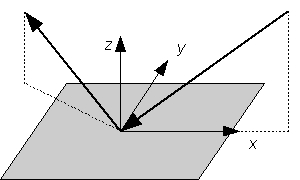
\includegraphics[height=40mm]{figs/sda/4_sda.jpg}

        As each photon is incident on the surface, it hits a random microscopic
        plate, and is reflected accordingly. The orientation of each plate is
        determined by the following algorithm:

        \begin{enumerate}
        \item Rotate the plate about the z{}-axis by some angle  $\theta _{z}$
        with uniform distribution on  $0\leqslant \theta _{z}<\pi $
        \item Rotate the plate about the \textit{rotated} x{}-axis by
        some angle $\theta _{x}$ with normal distribution
        with mean 0 and standard deviation determined by the desired
        ``roughness'' of the surface.
        \end{enumerate}

        Define:

         $\hat{i},\hat{j},\hat{k}$ The unit vectors defined by
        the coordinate system above

         $\hat{p}$ to be the unit vector directed \textit{against }the
         incident radiation

         $\hat{s}$ to be the unit vector associated with the reflected
         radiation, and \textit{x, y, }and\textit{ z }by
         $\hat{s}=x\hat{i}+y\hat{j}+z\hat{k}$

         $\hat{n}$ to be the unit vector normal to the plate

         $\phi $ to be the angle between  $\hat{k}$
         and $\hat{p}$

         $\hat{s}=x\hat{i}+y\hat{j}+z\hat{k}$ can be found in terms of  $\theta
         _{x}$ and  $\theta _{z}$ by the method following.

         \bigskip

         The original reference frame, \textit{O,} is rotated to a new
         reference frame, \textit{O'}, such that the surface normal is
         oriented along $\hat{k}\text{'}$ , the local z{}-axis in
         \textit{O'}.  The axes in
         \textit{O'} can be expressed in terms of the
         angles $\theta _{x}$ and  $\theta _{z}$ so that

         $\begin{gathered}\hat{i}\text{{\textquotesingle}}=\ \cos \theta
         _{z}\hat{i}+\sin \theta _{z}\hat{j}\hfill
         \\\hat{j}\text{{\textquotesingle}}=-\cos \theta _{x}\sin \theta
         _{z}\hat{i}+\cos \theta _{x}\cos \theta _{z}\hat{j}+\sin \theta
         _{x}\hat{k}\hfill \\\hat{k}\text{{\textquotesingle}}=\ \sin \theta
         _{x}\sin \theta _{z}\hat{i}-\sin \theta _{x}\cos \theta
         _{z}\hat{j}+\cos \theta _{x}\hat{k}\hfill \end{gathered}$

         Thus the transformation matrix representing the rotation from
         \textit{O} to \textit{O'} is

         $\left[\begin{matrix}\cos \theta _{z}&\sin \theta _{z}&0\\-\cos
         \theta _{x}\sin \theta _{z}&\cos \theta _{x}\cos \theta _{z}&\sin
         \theta _{x}\\\sin \theta _{x}\sin \theta _{z}&-\sin \theta _{x}\cos
         \theta _{z}&\cos \theta _{x}\end{matrix}\right]$

         \bigskip

         Thus, the vector  $\vec{p}$ can be transformed into \textit{O'}. In
         \textit{O'}, the beam is reflected in the
         local x{}-y plane at the origin, so
         $\hat{s}\text{{\textquotesingle}} = \left[\begin{matrix}s_{1}
         \text{'}\\s_{2}\text{'}\\s_{3}\text{'}\end{matrix} \right] =
         \left[\begin{matrix}-p_{1}\text{'}\\-p_{2}\text{'}\\p_{3}\text{'}
         \end{matrix} \right]$


         Then this can be transformed back into the frame
         \textit{O} by the transpose of the rotation matrix to produce the
         unit vector:

          $\hat{s}=\left[\begin{matrix}\sin \phi (2\sin ^{2}\theta
         _{x}\sin ^{2}\theta _{z}-1)+\cos \phi (2\sin \theta _{x}\cos \theta
         _{x}\sin \theta _{z})\\\sin \phi (-2\sin ^{2}\theta _{x}\sin \theta
         _{z}\cos \theta _{z})+\cos \phi (-2\sin \theta _{x}\cos \theta _{x}\cos
         \theta _{z})\\\sin \phi (2\sin \theta _{x}\cos \theta _{x}\sin \theta
         _{z})+\cos \phi (\cos ^{2}\theta _{x}-\sin ^{2}\theta
         _{x})\end{matrix}\right]$

         \bigskip

         Integrating over all values of $\theta_x$ and $\theta_z$, weighted
         by the respective probability
         functions

         \begin{equation*}
         p(\theta_z) = \frac{1}{\pi} d\theta_z
         \end{equation*}

         \begin{equation*}
         p(\theta_x) = \sqrt {\frac{c}{\pi}} \left( e^{-c {\theta_x}^2} \right) d \theta_x
         \end{equation*}

          produces an expected value

         \begin{equation}
           \langle \hat{s}\rangle =\left[\begin{matrix}-0.5\;\sin \phi
           \;\left(1+e^{-\frac{1}{c}}\right)\\0\\\cos \phi
           \;e^{-\frac{1}{c}}\end{matrix}\right]
           \label{eqn:s_hat_average}
        \end{equation}

         The value \textit{c} in the above expressions is a measure of the
         ``smoothness'' of the surface; a small value \textit{c} tends to a
         uniform distribution on $\theta_x$, indicative of a rough surface,
         while a large value of \textit{c} tends to produce a delta distribution
         on $\theta_x$ (i.e. all parallel to the surface), indicative of a smooth
         surface.

         Note that the average of unit vectors will typically not be a unit
         vector; this value is not a unit vector.

         This value also includes photons reflected ``down'' into the
         surface, which should undergo subsequent reflections until either
         absorbed or reflected out.

         Instead of using this value for the calculation of the force due to
         reflection, the value was numerically simulated by firing 10
         \textsuperscript{6} photons at the surface and tracking each photon
         until it was either absorbed, or reflected out.
         For code validation, this process was changed slightly so that all
         down{}-reflected photons were ignored, and instead re-calculated as
         newly incident photons; these results matched the analytic
         solution to better than 0.5\%.
         The differences observed when the effect of multiple
         reflections is included is seen mostly on the z{}-axis, and
         increases with both the incident angle, $\phi $  and the
         ``smoothness'' factor, \textit{c}.  The results of this
         investigation can be found in the section \textref{Validation of
         Flux-Vehicle Interaction-Model Principles}
         {test:flux_vehicle_interaction}.


         The incremental force added to the surface by a photon is

         \begin{equation*}
         \vec{\mathit{dF}}=\left\{\begin{matrix}\phi _{\gamma
         }\left(-\hat{p}-\hat{s}\right)\ \ \ \ \ \ \ \mathit{reflection}\\\phi
         _{\gamma
         }\left(-\hat{p}-\frac{2}{3}\hat{k}\right)\ \ \
         \mathit{absorption}\end{matrix}\right\}
         \end{equation*}


         and the total force
         \begin{equation}
           \vec{F}=\sum _{i=1}^{i=N}\vec{\mathit{dF}}_{i}
           \label{eqn:force_plate}
         \end{equation}


         The simplifying model used here, that avoids individual photon
         mapping, assumes that some fraction  $\alpha $ is
         reflected form the plane of the whole surface, of which some fraction
         $\delta $ is reflected totally diffusely and
         $1-\delta $ is reflected purely specularly. The
         balance $(1-\alpha )$ is absorbed and re{}-emitted.
         The re{}-emission profile is assumed to be Lambertian, as is the
         diffuse reflection profile. \

         The unit vectors  $\hat{p}$ and
         $\hat{s}$ have the same meaning as before, with

         $\hat{p}=\sin \phi \hat{i}+\cos \phi \hat{k}$

         $\hat{s}=-\sin \phi \hat{i}+\cos \phi \hat{k}$

         The total force then is

\begin{equation*}
         \vec{F}=N\phi _{\gamma }\left(-\hat{p}-\alpha (1-\delta
         )\hat{s}-\frac{2}{3}(1-\alpha (1-\delta ))\hat{k}\right)
\end{equation*}

          Note: under the assumption of thermal equilibrium, there is no
          distinction to be made between the force{}-expression associated with
          diffuse reflection and that with absorption/emission.  The force
          equation can therefore be simplified by saying some fraction
          $\sigma $ is reflected specularly:
          \begin{equation}
            \vec{F}=N\phi
            _{\gamma }\left(\hat{i}(\sin \phi )(\sigma -1)+\hat{k}\left((\sigma
            -1)\left(\frac{2}{3}-\cos \phi \right)-2\cos \phi \right)\right)
            \label{eqn:force_model}
          \end{equation}

          The value $\sigma $ can now be found as the
          value that minimizes the error between the two forces (equations
          \ref{eqn:force_plate} and \ref{eqn:force_model})

          The value $\alpha $ can be found from a count
          of the number of absorbed and reflected photons in the microscopic
          plate model,

          \begin{equation*}
          \alpha =\frac{n_{\mathit{reflected}}}{n_{\mathit{photons}}}.
          \end{equation*}

          The value $\delta $ can be found from $\alpha $ and $\sigma $ .

          A validation of this model can be found in section
          \textref{Validation of Flux-Vehicle Interaction-Model Principles}
          {test:flux_vehicle_interaction}.

  \subsection{Response of Temperature and Thermal Emission to Incident Flux}
  \label{sec:mathform_temp_resp}

    \subsubsection{Temperature Variation}
      Without a source of incident energy, the object should cool by
      radiation, according to

      \begin{equation}
        C\frac{\mathit{dT}}{\mathit{dt}}=-\epsilon A\sigma T^{4}
      \end{equation}

      where \textit{C} represents the heat capacity,
      $\epsilon $ the emissivity ,  $\alpha $ the albedo,
      \textit{ A} the emitting area,
      $\sigma $ the Stefan{}-Boltzmann constant, and
      \textit{T} the temperature.

      $\alpha$ and $\epsilon$ are surface dependent values, and must
      be included as part of the plate model.

      The analytic solution to this expression is

      \begin{equation}
        T(t)=\frac{T_{0}}{\sqrt[{3}]{1+3\left(\frac{\epsilon \sigma
        A}{C}\right)\;(T_{0})^{3}\;t}}
      \end{equation}

      with  $T(0)=T_{0}$

      The simulation is tested against this analytic result in section
      \vref{test:temperature}.

      There is no closed{}-form analytic solution for the case of an
      illuminated plate.

      For the temperature response under illumination, we first consider
      the variation of the force due to thermal emission, described  in
      the next subsection.

    \subsubsection{Variation of Force due to Thermal Emission}

      The force due to emission can be calculated from the magnitude of the
      momentum carried away with the
      emission in the direction of that emission, which is given by
      \begin{equation*}
      \frac{1}{c}\frac{\mathit{dE}}{\mathit{dt}},
      \end{equation*}

      Thus,
      \begin{equation}
        \vec{F}=\frac{2}{3}\frac{1}{c}\frac{\mathit{dE}}{\mathit{dt}}(-\hat{n})
      \end{equation}

      with \textit{c} representing the speed of light,
      \textit{E} the energy, and  $\hat{n}$ the normal to the plate surface.


      Due to symmetry, the total vector momentum emitted will be in the
      direction of the normal vector. Because the emission is not
      unidirectional, there will be components of the emission with
      opposing momentum vectors oriented in the plane of the
      surface; consequently, the magnitude of the \textit{net}
      momentum emission will not be equal to the ratio of the
      \textit{total} energy emission to the speed
      of light.  Instead, we have to assume an emission profile; in
      this model, we assume a Lambertian profile for which the necessary factor
      to account for the difference is 2/3 (see subsection
      \ref{sec:mathform_pflux_resp_desc} for description
      of the Lambertian profile).

      The force on the plate is, of course, in the opposite direction to the
      emission.

      Then, continuing the assumption that the plate is not
      illuminated, the force exerted on the plate by its emission is

      \begin{equation}
         F=\frac{2\epsilon \;\sigma
         \;A\;{T_{0}}^{4}}{3c}\left(1+\frac{3\epsilon \;\sigma
         \;A}{C}\;(T_{0})^{3}t\right)^{-{\frac{4}{3}}}
      \end{equation}

      It should be recognized that the values of \textit{t} for the force and
      for the temperature are necessarily different due to the discretization
      of time in the simulation. The analytic expressions are valid for any
      particular time, \textit{t}, and this is sufficient for the
      temperature.  However, the force will be converted to acceleration,
      then integrated to provide velocity and position increments.
      Using the value of the force at either the beginning or end of a
      timestep, for the entire integration leads to errors; a more accurate
      representation would be to use some midpoint value. Instead, the
      force is
      calculated at time \textit{t} for the timestep from \textit{t
      }to\textit{ t+}\textit{${\Delta}$}\textit{t. } A closer
      approximation for the calculated force would be:

      \begin{equation}
        F(t\rightarrow t+\Delta t)\approx \frac{2\epsilon \;\sigma
        \;A\;{T_{0}}^{4}}{3c}\left(1+\frac{3\epsilon \;\sigma
        \;A}{C}\;(T_{0})^{3}\left(t+\frac{\Delta
        t}{2}\right)\right)^{-{\frac{4}{3}}}
      \end{equation}

      The simulation handles this problem by first integrating the temperature
      over the timestep using a Runge{}-Kutte 4\textsuperscript{th} order
      algorithm:

      The intermediate temperature deltas, $I_{1}, I_{2}, I_{3}, and I_{4}$
      are calculated by

      $I_{1}={\frac{\Delta t}{C}}\left( {\Pi-\epsilon A \sigma {T_{i}}^{4}}
      \right)$

      $I_{2}={\frac{\Delta t}{C}}\left( {\Pi-\epsilon A \sigma \left( {
      T_{i} + I_{1}/2} \right) ^{4} } \right)$

      $I_{3}={\frac{\Delta t}{C}}\left( {\Pi-\epsilon A \sigma \left( {
      T_{i} + I_{2}/2} \right) ^{4} } \right)$

      $I_{4}={\frac{\Delta t}{C}}\left( {\Pi-\epsilon A \sigma \left( {
      T_{i} + I_{3}} \right) ^{4} } \right)$

      and averaged to give

      $T_{i+1} = T_{i} + \left( \frac {I_{1}+2I_{2}+2I_{3}+I_{4}}{6}
      \right)$

      where
      \begin{itemize}
        \item{}$\Delta t$ is the timestep;
        \item{}$\sigma$ is the Stefan-Boltzmann constant; and
        \item{}C is the heat capacity,
        \item{}$\Pi$ is the power absorption rate from all sources,
        \item{}$\epsilon$ is the emissivity,
        \item{}A is the area, and
        \item{}$T_{i}$ is the starting temperature of the plate.
      \end{itemize}

      Then, using an energy balance,

      $C \Delta T = \left( \Pi - \xi \right) \Delta t$

      the rate at which energy is emitted, $\xi$, is
      calculated based on the temperature change and the energy absorbed
      during that timestep.

      This emitted energy is converted into a
      momentum, and multiplied by the 2/3 that results from the integration
      over the Lambertian emission profile to give a time{}-averaged
      force, valid over the entire timestep.

      \begin{equation}
        \langle \vec F \rangle = \frac{2}{3c}
        \left( \frac{C \Delta T}{\Delta t} -\Pi \right) \hat n
      \end{equation}


      Consequently, the routine
      \textit{thermal\_integrator} calculates the value corresponding to the
      energy balance over the timestep that is in turn used in the
      calculation of the emission force by routine
      \textit{radiation\_pressure.}



\subsection{Coefficient of Reflection}\label{sec:coefficientofreflection}

When using the single isotropic, isothermal, spherical, default surface,
there is the option to use a Coefficient of Reflection rather than the
combination of albedo and diffuse parameters.  This section describes how
that coefficient is used in the more general framework.

The concept of the Coefficient of Reflection is that the vehicle can be
modeled as a single, perfectly absorbing, flat plate, with some
\textit{effective area, A'} that is always oriented perpendicular to the flux
vector (i.e. its normal vector and the flux vector are anti-parallel).  To
obtain a constant area requires that the vehicle be modeled as a sphere,
so that its orientation cannot affect its projected area.

The physical dimensions of the vehicle can then be modeled with a single
parameter, the radius, \textit{R}.  The cross-sectional area that the
vehicle projects perpendicular to the flux vector is then $\pi R^2$.

In general, $A' \neq \pi R^2$.  The difference is due to the difference
between the reflective characteristics of the real surface and the assumed
perfect absorption of the simple surface.  That difference is modeled as
the Coefficient of Reflection, $C_R$:

\begin{equation*}
A' = C_R \pi R^2
\end{equation*}

Just as with the regular surface, developed in the Surface Model, the
simple surface can be considered to interact with the radiation field
through absorption, specular reflection, and diffuse reflection.

\subsubsection{Absorption}
The projected area absorbs everything that is incident upon it; the
projected area and
effective area are identical.  $C_R = 1.0$

\subsubsection{Specular Reflection}
Figure \ref{fig:defaultsurfacespecular} shows a representation of a
sphere, illuminated from the right, with three light rays added showing
the paths due to specular reflection.

\begin{figure}[!ht]
\begin{center}
    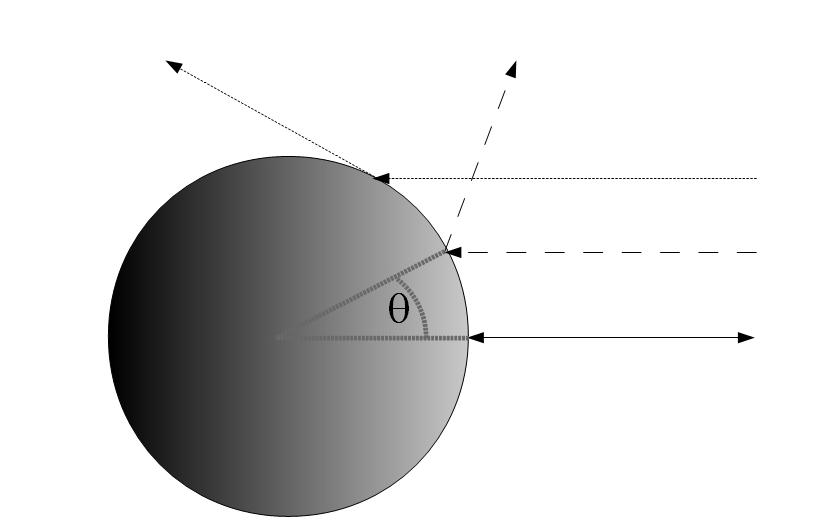
\includegraphics[height=60mm]{figs/def_surf/specular.jpg}
    \end{center}
    \caption{Light Rays Incident on a Specular Spherical Surface}
    \label{fig:defaultsurfacespecular}
  \end{figure}

One ray is reflected stright back, one is reflected at an angle close
to perpendicular to its incident path, and another is deflected very
little from its incident path.  For a photon hitting the surface at a
point that subtends some angle $\theta$ from the flux vector, the
reflected ray will be at angle $2 \theta$.  The momentum change of
the photon (defining the x-axis as being anti-parallel to the flux
vector) is then

\begin{equation*}
\Delta \vec{p} = p(\hat{i} + \cos 2\theta \hat{i} + \sin 2\theta \hat j)
\end{equation*}

where $p$ is the magnitude of the momentum of the photon.

Assuming that the sphere is uniformly illuminated (at least across
the illuminated side) leads to the argument that, by symmetry, the
forces off the x-axis will cancel to zero.

To obtain the force along the x-axis, consider dividing the sphere
into concentric rings, centered about $\theta = 0$.  For a small
range, $d\theta$, there will be a ring of elemental area
$(2 \pi R \sin \theta)(R d\theta)$.  This elemental area will
project, perpendicular to the flux vector, an area
$(2 \pi R^2 \sin \theta d \theta) \cos \theta$.

Therefore, the fraction of the projected disk resulting from the
sphere at some angle $\theta$ is

\begin{equation*}
\delta(\theta) = 2 \sin \theta \cos \theta d \theta = \sin 2 \theta d \theta
\end{equation*}

This is the fraction of the total flux that is incident at any
particular angle $\theta$.

The force due to specular reflection is then

\begin{equation*}
\vec F = \vec \phi \pi R^2 \int_{0}^{\pi/2} (1 + \cos 2\theta) sin 2\theta d\theta
\end{equation*}

where $\vec \phi$ is the momentum flux vector ($N cdot m^{-2}$).

The somewhat surprising result of this integration is that

\begin{equation*}
\vec F = - \vec \phi \pi R^2
\end{equation*}

i.e., the specular sphere behaves exactly the same as a perfectly
absorbing sphere, and therefore has $C_R = 1.0$.

While this may not be expected, it is logical with further consideration.
The photons incident very close to the edge of the sphere will
continue almost unaffected, resulting in minimal force on the
sphere.  Conversely, the photons incident near the center will
be reflected back on the same path, resulting in twice the force
that they would produce if absorbed.  Those incident with
$\theta = 45 ^o$ will exert exactly the same force (along
the x-axis) on the sphere as they would exert if absorbed.
Therefore, the photons hitting inside 45 degrees exert additional
force, those outside 45 degrees exert less force, with nice symmetry.
Integrating the projected area for $0 \leqslant \theta < 45^o$ and
for $45 < \theta \leqslant 90^o$ yields the same value; the deficit
resulting from those photons outside the 45 degree circle balances
with the excess from those inside the circle.

\subsubsection{Diffuse Reflection}
The diffuse reflection is handled using a Lambertian profile and the
same mathematical methods as in the previous section.

\begin{equation*}
\vec F = \vec \phi \pi R^2 \int_{0}^{\pi/2} \left(1 + \frac{2}{3} \cos \theta \right) sin 2\theta d\theta = \frac{13}{9} \vec \phi \pi R^2
\end{equation*}

i.e., the diffuse sphere produces a larger force than would a specular
or absorbing sphere of the same size, and has $C_R = \frac{13}{9}$.

\subsubsection{Composite Surface}
Combining the three processes together yields

\begin{equation}
C_R = (1-\alpha) + \alpha(1-\delta) + \frac{13}{9} \alpha \delta  = 1 + \frac{4}{9} \alpha \delta \in[1.0,1.444]
\end{equation}
where $\alpha$ is the albedo and $\delta$ is the diffuse parameter.

Note that there is a one-to-many relation between the values of
$C_R$ and the values of $\alpha, \delta$.

The code continues to use $\alpha$ and $\delta$; when a user
specifies a coefficient, it is converted into

$\alpha =\frac{9}{4} (C_R - 1)$ and $\delta = 1 $
